%! Author = gramic
%! Date = 08.04.24

% Preamble
\begin{flushleft}
    \subsection{Testing Evaluationssysteme}
    %%! Author = gramic
%! Date = 08.04.24

% Preamble
\begin{flushleft}
    \subsubsection{Evaluation - Testfälle}
    \paragraph{Patroni}
    \begin{description}
        \item \textbf{Failover}\hfill \\
        \begin{enumerate}
            \item Der Server des Primary-Node wird manuell heruntergefahren.
            \item Während dem Failover müssen Daten via SQL\\eingeführt und ausgelesen werden.
            \item Während dem Failover muss mindestens eine längere Abfrage gestartet werden.
        \end{enumerate}
        \item \textbf{Switchover}\hfill \\
%        \setcounter{enumi}{4}
        \begin{enumerate}[resume]
            \item Mit der REST-API wird der Switchover\\auf einen anderen Nod abgesetzt.
            \item Mit dem \texttt{patronictl}-Command wird der Switchover gesetzt
            \item Während dem Switchover müssen Daten via SQL\\eingeführt und ausgelesen werden.
            \item Während dem Switchover muss mindestens eine längere Abfrage gestartet werden.
        \end{enumerate}
        \item \textbf{Restore}\hfill \\
%        \setcounter{enumi}{9}
        \begin{enumerate}[resume]
            \item Mit der REST-API wird der Node erst mit dem \texttt{reinitialize} wiederhergestellt\\und dann mit einem Switchover wieder als Primary gesetzt.
            \item Mit dem \texttt{patronictl}-Commandund Parameter \texttt{reinit} der Node wiederhergestellt\\und abschliessend mittels Switchover wieder als Primary gesetzt.
            \item Mit der REST-API wird der Node mit dem \texttt{reinitialize} wiederhergestellt
            \item Mit dem \texttt{patronictl}-Commandund Parameter \texttt{reinit} der Node wiederhergestellt
            \item Vor, während und nach dem Restore müssen Tabellen mit Foreign-Key-Constraints und Daten geprüft werden.
            \item Während dem Restore muss mindestens eine längere Abfrage gestartet werden und Daten via SQL\\eingeführt und ausgelesen werden.
        \end{enumerate}
    \end{description}
    \paragraph{StackGres - Citus}
    \begin{description}
        \item \textbf{Failover}\hfill \\
        \begin{enumerate}
            \item Der Server des Leader-Cooordinator-Node wird manuell heruntergefahren.
            \item Während dem Failover müssen Daten via SQL\\eingeführt und ausgelesen werden.
            \item Während dem Failover muss mindestens eine längere Abfrage gestartet werden.
        \end{enumerate}
        \item \textbf{Sharding}\hfill \\
%        \setcounter{enumi}{4}
        \begin{enumerate}[resume]
            \item Vor, während und nach dem Failover müssen Tabellen mit Foreign-Key-Constraints geprüft werden.
            \item Nach einem Failover-Test müssen alle Daten vorhanden sein.
        \end{enumerate}
        \item \textbf{Self Healing}\hfill \\
        \begin{enumerate}[resume]
            \item Der Node muss wieder hochgefahren werden.\\Der Node muss selbstständig Daten synchronisieren.
            \item Der Leader muss automatisch neu gesetzt werden, wenn notwendig
        \end{enumerate}
    \end{description}
    \paragraph{YugabyteDB}
    \begin{description}
        \item \textbf{Failover}\hfill \\
        \begin{enumerate}
            \item Ein k8s Node wird manuell heruntergefahren,\\indem der entsprechende Server heruntergefahren wird.
            \item Während dem Failover müssen Daten via SQL\\eingeführt und ausgelesen werden.
            \item Während dem Failover muss mindestens eine längere Abfrage gestartet werden.
        \end{enumerate}
        \item \textbf{Sharding}\hfill \\
%        \setcounter{enumi}{4}
        \begin{enumerate}[resume]
            \item Vor, während und nach dem Failover müssen Tabellen mit Foreign-Key-Constraints geprüft werden.
            \item Nach einem Failover-Test müssen alle Daten vorhanden sein.
        \end{enumerate}
        \item \textbf{Self Healing}\hfill \\
        \begin{enumerate}[resume]
            \item Der Node muss wieder hochgefahren werden.\\Der Node muss selbstständig Daten synchronisieren.
        \end{enumerate}
    \end{description}
\end{flushleft}
\begin{flushleft}
    \subsubsection{Evaluation - ERD self\_healing\_test}
    \label{subsubsec:erd_self_healing_test}
    Die Tests müssen bei allen drei Varianten anhand der Datenbank \texttt{self\_healing\_test} durchgeführt werden.\\
    Dabei werden die Tabellen, im hinblick auf das Citus Schema Based Sharding, in Schemas organisiert.\\
    Zwischen den einzelnen Schemas sollen einige Tabellen einen Foreign-Key auf andere Tabellen legen:
    \begin{figure}[H]
        \centering
        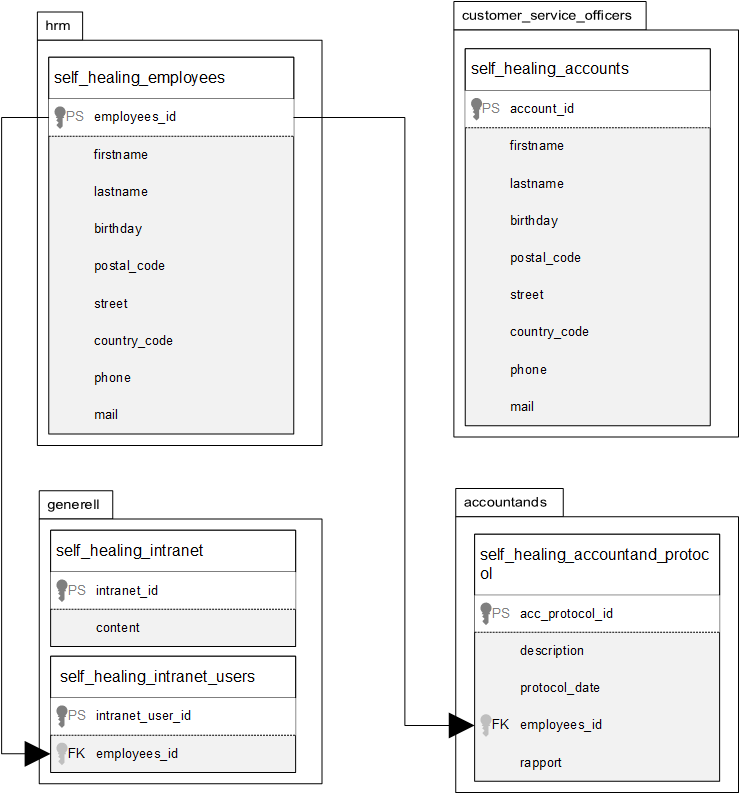
\includegraphics[width=0.5\linewidth]{source/implementation/evaluation/evaluation_tests/erd_self_healing_test}
        \caption{Testing - ERD DB self\_healing\_test}
        \label{fig:erd_self_healing_test}
    \end{figure}
\end{flushleft}
    %%! Author = gramic
%! Date = 15.03.24

% Preamble
\begin{flushleft}
    \subsubsection{yugabyteDB}
    \paragraph{Installation}
    Wähend der Installation des YugabyteDB Evaluations-Enviroment wurde festgestellt, das man zwei Varianten Installieren kann.
    YugabyteDB (Repository yugabyte) und YugabyteDB Anywhere (Repository yugawre):
    \begin{figure}[H]
        \centering
        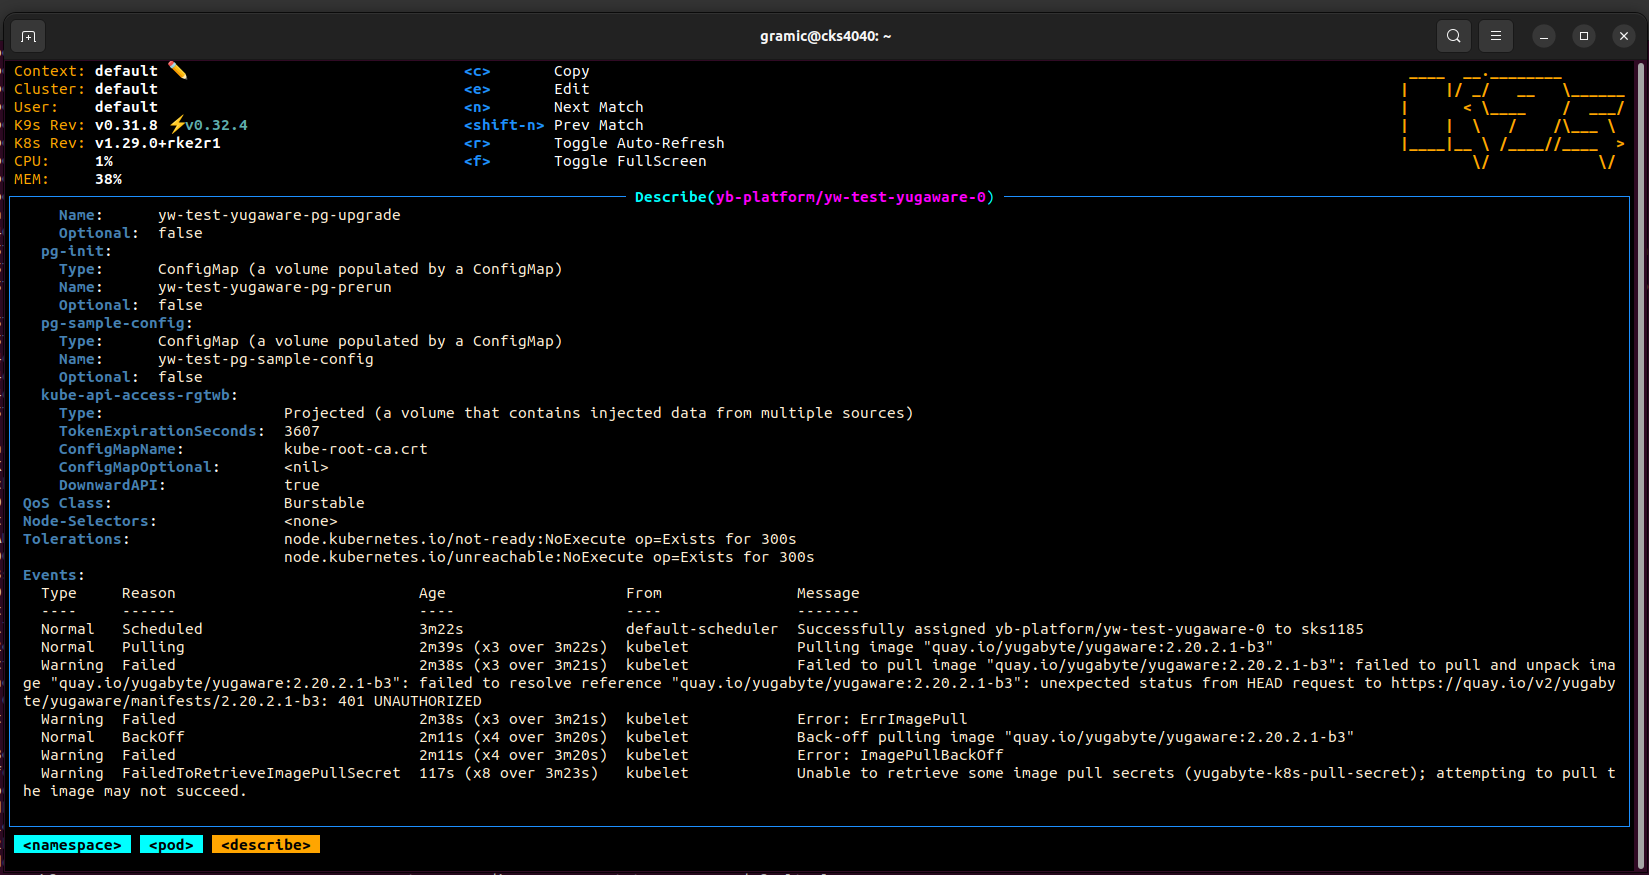
\includegraphics[width=1\linewidth]{source/implementation/evaluation/platforms/yugabytedb_pod_installation_subscription_interrup}
        \caption{yugabyteDB - Susbsription yugawre}
        \label{fig:yugabytedb_pod_installation_subscription_interrup}
    \end{figure}
\end{flushleft}
\begin{flushleft}
    Es stellte sich auch heraus, dass wenn man YugabyteDB 4 Cores pro Node zur Verfügung geben will (je zwei für den \texttt{master} und \texttt{tserver}),\\
    der Server mehr als 4 Cores haben muss.\\
    Andernfalls wird Kubernetes einen der beiden Pods nicht deployen, weil zuwenig Cores zur verfügung stehen.
\end{flushleft}
\begin{flushleft}
    Bei der konstelation \gls{rke2}, \Gls{Cilium} und \Gls{MetalLB}, muss nebst dem \texttt{IPAddressPool} auch ein \texttt{L2Advertisement} für den Pool gesetzt werden.\\
    Ansonsten kann die im YugabyteDB values.yaml gesetzte IP für den \texttt{tserver} von aussen nicht angesprochen werden:
    \lstset{style=gra_codestyle}
    \begin{lstlisting}[language=yaml, caption=metallb - Konfig YAML - Detail L2Advertisement,captionpos=b,label={lst:metallb-l2advertisement-setting},breaklines=true]
---
apiVersion: metallb.io/v1beta1
kind: L2Advertisement
metadata:
  name: l2adv
  namespace: metallb-system
spec:
  ipAddressPools:
  - distributed-sql
    \end{lstlisting}
    Dieses Problem ist schwer zu greifen und hat zwei Tage in Anspruch genommen, es zu Lösen.
    Die Vorschläge zum Lösen des Problems reichten von deakivieren von \texttt{kube-proxy} bis hin zu einer Migration zum \Gls{Cilium}-Loadb-Balancers.\\
    Mit diesem funktionierte dann nicht einmal mehr die Installation von yugabyteDB.\\
    Lösung brachte nur ein \texttt{GitHub}-Eintrag\cite{D4IZIEFN}, wo oben genannter Ansatz empfohlen wurde.
\end{flushleft}
\begin{flushleft}
    \paragraph{Konfiguration}
    Damit nicht der YugabyteDB Anywhere-Service installiert wird, muss das entsprechende Image gesetzt werden:
    \lstset{style=gra_codestyle}
    \begin{lstlisting}[language=yaml, caption=yugabyteDB - Helm Chart Manifest - Detail Image,captionpos=b,label={lst:yugabytedb-image-setting},breaklines=true]
...
Image:
  repository: "yugabytedb/yugabyte"
  tag: 2.20.2.1-b3
  pullPolicy: IfNotPresent
  pullSecretName: ""
...
    \end{lstlisting}

    Die StorageClass muss im \texttt{values.yaml} gesetzt werden, einmal für den \texttt{master} und einmal für den \texttt{tserver}
    \lstset{style=gra_codestyle}
    \begin{lstlisting}[language=yaml, caption=yugabyteDB - Helm Chart Manifest - Detail StorageClass,captionpos=b,label={lst:yugabytedb-storageclass-setting},breaklines=true]
...
storage:
  ephemeral: false  # will not allocate PVs when true
  master:
    count: 1
    size: 3Gi
    storageClass: "yb-storage"
  tserver:
    count: 1
    size: 3Gi
    storageClass: "yb-storage"
...
    \end{lstlisting}

    Dem node werden je 4 Cores zur verfügung gestellt.
    Zei für den \texttt{master} und zwei für den \texttt{tserver}.
    Beide erhalten 4GiB Memory:
    \lstset{style=gra_codestyle}
    \begin{lstlisting}[language=yaml, caption=yugabyteDB - Helm Chart Manifest - Detail Resources,captionpos=b,label={lst:yugabytedb-resources-setting},breaklines=true]
...
resource:
  master:
    requests:
      cpu: "1"
      memory: 2Gi
    limits:
      cpu: "1"
      ## Ensure the 'memory' value is strictly in 'Gi' or 'G' format. Deviating from these formats
      ## may result in setting an incorrect value for the 'memory_limit_hard_bytes' flag.
      ## Avoid using floating numbers for the numeric part of 'memory'. Doing so may lead to
      ## the 'memory_limit_hard_bytes' being set to 0, as the function expects integer values.
      memory: 2Gi
  tserver:
    requests:
      cpu: "1"
      memory: 4Gi
    limits:
      cpu: "1"
      ## Ensure the 'memory' value is strictly in 'Gi' or 'G' format. Deviating from these formats
      ## may result in setting an incorrect value for the 'memory_limit_hard_bytes' flag.
      ## Avoid using floating numbers for the numeric part of 'memory'. Doing so may lead to
      ## the 'memory_limit_hard_bytes' being set to 0, as the function expects integer values.
      memory: 4Gi
...
    \end{lstlisting}

    Die Shards, oder Tablets wie sie Yugabyte nennt, sollen auf allen drei Nodes repliziert werden:
    \lstset{style=gra_codestyle}
    \begin{lstlisting}[language=yaml, caption=yugabyteDB - Helm Chart Manifest - Detail Replika,captionpos=b,label={lst:yugabytedb-replica-setting},breaklines=true]
...
replicas:
  master: 3
  tserver: 3
  ## Used to set replication factor when isMultiAz is set to true
  totalMasters: 3
...
    \end{lstlisting}

    Wichtig ist auch, dass der \texttt{YSQL}-Dienst aktiv ist, damit PostgreSQL Abfragen abgesetzt werden können.\\
    Deshalb muss der Dienst aktiv sein und darf nicht deaktiviert werden:
    \lstset{style=gra_codestyle}
    \begin{lstlisting}[language=yaml, caption=yugabyteDB - Helm Chart Manifest - Detail Disable YSQL,captionpos=b,label={lst:yugabytedb-disableYsql-setting},breaklines=true]
...
# Disable the YSQL
disableYsql: false
...
    \end{lstlisting}

    Nun muss die Domain und die Service-Endpoints konfiguriert werden.\\
    Der Domainname bleibt vorerst \texttt{cluster.local} wie Default hinterlegt.\\
    Die Servicenamen und Ports werden nicht angetastet, wichtig ist die LoadBalancer-IP.\\
    Sie ist entsprechend der gewählten VirtualIP mit \texttt{10.0.20.106} zu setzen.

    \lstset{style=gra_codestyle}
    \begin{lstlisting}[language=yaml, caption=yugabyteDB - Helm Chart Manifest - Detail Domainname und Service-Endpoints,captionpos=b,label={lst:yugabytedb-domainname-serviceendpoints-setting},breaklines=true]
...
domainName: "cluster.local"

serviceEndpoints:
  - name: "yb-master-ui"
    type: LoadBalancer
    annotations: {}
    clusterIP: ""
    ## Sets the Service's externalTrafficPolicy
    externalTrafficPolicy: ""
    app: "yb-master"
    loadBalancerIP: ""
    ports:
      http-ui: "7000"

  - name: "yb-tserver-service"
    type: LoadBalancer
    annotations:
      metallb.universe.tf/loadBalancerIPs: 10.0.20.106
    clusterIP: ""
    ## Sets the Service's externalTrafficPolicy
    externalTrafficPolicy: ""
    app: "yb-tserver"
    loadBalancerIP: ""
    ports:
      tcp-yql-port: "9042"
      tcp-yedis-port: "6379"
      tcp-ysql-port: "5433"
...
    \end{lstlisting}
\end{flushleft}
\begin{flushleft}
    Beim Testen mit der höchsten Anzahl an Datensätzen zeigte sich, dass der \gls{local-path-provisioner} nicht sauber konfiguriert waren.\\
    Damit auf jedem Node die Persistence Volume Claims ausgeführt werden, müssen sie deklariert werden und in den StorageClass-Manifesten auch hinterlegt werden.\\
    Genauer muss in der \texttt{nodePathMap} folgende konfiguration vorgenommen werden:
\lstset{style=gra_codestyle}
\begin{lstlisting}[language=yaml, caption=local-path-provisioner nodePathMap,captionpos=b,label={lst:local-path-provisioner_nodePathMap},breaklines=true]
...
                "nodePathMap":[
                {
                        "node":"DEFAULT_PATH_FOR_NON_LISTED_NODES",
                        "paths":["<Lokaler Pfad>"]
                },
                {
                        "node":"<Nodename>",
                        "paths":["<Lokaler Pfad>"]
                },
...
\end{lstlisting}
    Hier ein Beispiel wie es mit den grossen Volumes aussieht:
\lstset{style=gra_codestyle}
\begin{lstlisting}[language=yaml, caption=local-path-provisioner nodePathMap Beispiel,captionpos=b,label={lst:local-path-provisioner_nodePathMap-exampl},breaklines=true]
...
                "nodePathMap":[
                {
                        "node":"DEFAULT_PATH_FOR_NON_LISTED_NODES",
                        "paths":["/srv/data/local-path-provisioner"]
                },
                {
                        "node":"sks1183",
                        "paths":["/srv/data/local-path-provisioner"]
                },
                {
                        "node":"sks1184",
                        "paths":["/srv/data/local-path-provisioner"]
                },
                {
                        "node":"sks1185",
                        "paths":["/srv/data/local-path-provisioner"]
                }
                ]
...
\end{lstlisting}
    Wird dies nicht gemacht, so wird auf den Default-Path geschrieben.\\
    Das ist zufällig und hat dann zur Folge, dass alle Volumes auf einem Node präsentiert werden.\\
    Was sehr schnell logischerweise dazu führt, dass zuwenig Diskspace vorhanden ist.\\
    Bei YugabyteDB kommt noch dazu, dass es zu Konflikten beim Schreiben von Blocks kommt.
\end{flushleft}
\begin{flushleft}
    Damit die Persistence Volumes sauber präsentiert werden, muss in der StorageClass die \texttt{nodeAffinity} gesetzt werden.\\
    Hier als Beispiel mit den Nodes \texttt{sks1183}, \texttt{sks1184} und \texttt{sks1185}:
\lstset{style=gra_codestyle}
\begin{lstlisting}[language=yaml, caption=yugabyteDB - StorageClass nodeAffinity,captionpos=b,label={lst:yugabytedb-storageclass_example},breaklines=true]
  nodeAffinity:
    required:
      nodeSelectorTerms:
      - matchExpressions:
        - key: kubernetes.io/hostname
          operator: In
          values:
          - sks1183
          - sks1184
          - sks1185
\end{lstlisting}
    \begin{warning}
        \textbf{hostPath}\\
        Der \texttt{hostPath} bei der StorageClass muss der gleiche sein, wie der Pfad im Node des nodePathMap von \gls{local-path-provisioner}.
        Auch sollten die Pfade auf allen Nodes gleich sein.
    \end{warning}
\end{flushleft}
\begin{flushleft}
    Die Problematik mit dem \texttt{nodePathMap} und der \texttt{nodeAffinity} auf der StorageClass hat auch rund zwei Arbeitstage in Anspruch genommen.
\end{flushleft}
    \subsubsection{Patroni}
    \begin{table}[H]

\resizebox{\columnwidth}{!}{%

\begin{tabular}{lrllll}
\toprule
Art & Test Case Nr. & Test Case & Erwartetes Ergebnis & Eingetretenes Ergebnis & Begründung \\
\midrule
Failover & 1 & Automatismus & \begin{tabular}[c]{@{}l@{}}Wird der Primary Server vom Netz genommen,\\führt Patroni einen Failover auf einen Replika-Node\end{tabular} & \begin{tabular}[c]{@{}l@{}}Eingetroffen\end{tabular} & \begin{tabular}[c]{@{}l@{}}\end{tabular} \\
Failover & 2 & Connection-Stabilität & \begin{tabular}[c]{@{}l@{}}Bestehende Connections dürfen nicht getrennt werden.\end{tabular} & \begin{tabular}[c]{@{}l@{}}Nicht eingetroffen\end{tabular} & \begin{tabular}[c]{@{}l@{}}Connection-Stabilität kann nur hergestellt werden,\\wenn entweder die Applikation dazu in der Lage ist\\oder man einen Connection-Pooler wie pgBouncer einsetzt.\\Es wurde aber keiner eingesetzt.\end{tabular} \\
Failover & 3 & Geschwindigkeit & \begin{tabular}[c]{@{}l@{}}Der Failover muss so schnell stattfinden,\\dass offene Connections nicht wegen eines Timeouts geschlossen werden.\end{tabular} & \begin{tabular}[c]{@{}l@{}}Bedingt eingetroffen\end{tabular} & \begin{tabular}[c]{@{}l@{}}Auch hier hängt die stabilität an den Settings der Applikation\\und oder einem Connection-Pooler.\end{tabular} \\
Switchover & 4 & Skript / API & \begin{tabular}[c]{@{}l@{}}Mit der Patroni REST-API wird der Switchover ausgeführt\end{tabular} & \begin{tabular}[c]{@{}l@{}}Eingetroffen\end{tabular} & \begin{tabular}[c]{@{}l@{}}\end{tabular} \\
Switchover & 5 & Skript / API & \begin{tabular}[c]{@{}l@{}}Mit dem Patroni Commandset wird er Switchover ausgeführt\end{tabular} & \begin{tabular}[c]{@{}l@{}}Eingetroffen\end{tabular} & \begin{tabular}[c]{@{}l@{}}\end{tabular} \\
Switchover & 6 & Connection-Stabilität & \begin{tabular}[c]{@{}l@{}}Bestehende Connections dürfen nicht getrennt werden.\end{tabular} & \begin{tabular}[c]{@{}l@{}}Eingetroffen\end{tabular} & \begin{tabular}[c]{@{}l@{}}\end{tabular} \\
Switchover & 7 & Geschwindigkeit & \begin{tabular}[c]{@{}l@{}}Der Switchover muss so schnell stattfinden,\\dass offene Connections nicht wegen eines Timeouts geschlossen werden.\end{tabular} & \begin{tabular}[c]{@{}l@{}}Nicht eingetroffen\end{tabular} & \begin{tabular}[c]{@{}l@{}}Connection-Stabilität kann nur hergestellt werden,\\wenn entweder die Applikation dazu in der Lage ist\\oder man einen Connection-Pooler wie pgBouncer einsetzt.\\Es wurde aber keiner eingesetzt.\end{tabular} \\
Restore & 9 & Skript / API & \begin{tabular}[c]{@{}l@{}}Mit der Patroni REST-API wird der Primary-Node Wiederhergestellt\end{tabular} & \begin{tabular}[c]{@{}l@{}}Eingetroffen\end{tabular} & \begin{tabular}[c]{@{}l@{}}\end{tabular} \\
Restore & 10 & Skript / API & \begin{tabular}[c]{@{}l@{}}Mit dem Patroni Commandset der Primary-Node Wiederhergestellt\end{tabular} & \begin{tabular}[c]{@{}l@{}}Eingetroffen\end{tabular} & \begin{tabular}[c]{@{}l@{}}\end{tabular} \\
Restore & 11 & Skript / API & \begin{tabular}[c]{@{}l@{}}Mit der Patroni REST-API wird ein Replika-Node Wiederhergestellt\end{tabular} & \begin{tabular}[c]{@{}l@{}}Eingetroffen\end{tabular} & \begin{tabular}[c]{@{}l@{}}\end{tabular} \\
Restore & 12 & Skript / API & \begin{tabular}[c]{@{}l@{}}Mit dem Patroni Commandset ein Replika-Node Wiederhergestellt\end{tabular} & \begin{tabular}[c]{@{}l@{}}Eingetroffen\end{tabular} & \begin{tabular}[c]{@{}l@{}}\end{tabular} \\
Restore & 13 & Datensicherheit & \begin{tabular}[c]{@{}l@{}}Beim Restore des Primary-Nodes dürfen keine Daten, \\die seit dem Failover gechrieben wurden,\\darf es zu keinem Datenverlust kommen\end{tabular} & \begin{tabular}[c]{@{}l@{}}Eingetroffen\end{tabular} & \begin{tabular}[c]{@{}l@{}}\end{tabular} \\
Restore & 14 & Connection-Stabilität & \begin{tabular}[c]{@{}l@{}}Beim Restore des Primary-Nodes dürfen keine Connections geschlossen werden.\end{tabular} & \begin{tabular}[c]{@{}l@{}}Nicht eingetroffen\end{tabular} & \begin{tabular}[c]{@{}l@{}}Connection-Stabilität kann nur hergestellt werden,\\wenn entweder die Applikation dazu in der Lage ist\\oder man einen Connection-Pooler wie pgBouncer einsetzt.\\Es wurde aber keiner eingesetzt.\end{tabular} \\
\bottomrule
\end{tabular}
}
\caption{Testresultate Evaluation Patroni} \label{evaluation_tests_patroni}
\end{table}

\end{flushleft}
\begin{flushleft}
    \subsubsection{StackGres -Citus}
    StackGres kann nicht alle Anforderungen erfüllen.
    Obwohl es mit \texttt{envoy} und \texttt{pgBounder} einen Proxy und einen Connection Pooler gibt,\\
    scheint dies nicht über die Coordinator-Nodes selbst zu gehen.\\
    Daher brechen bestehende Connections ab oder laufen irgendwann in ein Timeout, wenn \Gls{Kubernetes} Nodes nicht schnell genug heruntergefahren werden.
    \begin{table}[H]

\resizebox{\columnwidth}{!}{%

\begin{tabular}{lrllll}
\toprule
Art & Test Case Nr. & Test Case & Erwartetes Ergebnis & Eingetretenes Ergebnis & Begründung \\
\midrule
Failover & 1 & Automatismus & \begin{tabular}[c]{@{}l@{}}Wird der Primary Server vom Netz genommen,\\führt Patroni einen Failover auf einen Replika-Node\end{tabular} & \begin{tabular}[c]{@{}l@{}}Eingetroffen\end{tabular} & \begin{tabular}[c]{@{}l@{}}\end{tabular} \\
Failover & 2 & Connection-Stabilität & \begin{tabular}[c]{@{}l@{}}Bestehende Connections dürfen nicht getrennt werden.\end{tabular} & \begin{tabular}[c]{@{}l@{}}Nicht eingetroffen\end{tabular} & \begin{tabular}[c]{@{}l@{}}Keine.\\StackGres setzt envoy ein.\\Offensichtlich nicht ber einen ganzen Cluster\end{tabular} \\
Failover & 3 & Geschwindigkeit & \begin{tabular}[c]{@{}l@{}}Der Failover muss so schnell stattfinden,\\dass offene Connections nicht\\wegen eines Timeouts geschlossen werden.\end{tabular} & \begin{tabular}[c]{@{}l@{}}Nicht eingetroffen\end{tabular} & \begin{tabular}[c]{@{}l@{}}Keine.\\StackGres setzt envoy ein.\\Offensichtlich nicht ber einen ganzen Cluster\end{tabular} \\
Sharding & 4 & Datenkonsistenz\\und Datenintegrität & \begin{tabular}[c]{@{}l@{}}Daten sind Konsistent und Inetger.\end{tabular} & \begin{tabular}[c]{@{}l@{}}Eingetroffen\end{tabular} & \begin{tabular}[c]{@{}l@{}}\end{tabular} \\
Sharding & 5 & Schutz vor Datenverlust & \begin{tabular}[c]{@{}l@{}}Die Daten müssen Konsistent und schnell auf die Shards verteilt werden\end{tabular} & \begin{tabular}[c]{@{}l@{}}Eingtetroffen\end{tabular} & \begin{tabular}[c]{@{}l@{}}\end{tabular} \\
Self Healing & 6 & Node stellt sich selber wieder her & \begin{tabular}[c]{@{}l@{}}Shard Node wird automatisch synchronisiert\end{tabular} & \begin{tabular}[c]{@{}l@{}}Eingtetroffen\end{tabular} & \begin{tabular}[c]{@{}l@{}}\end{tabular} \\
Self Healing & 7 & Leader wird automatisch gesetzt & \begin{tabular}[c]{@{}l@{}}Leader wird entweder beibehalten\\oder wird neu gesetzt wenn ein Node zurückkehrt\end{tabular} & \begin{tabular}[c]{@{}l@{}}Eingetroffen\end{tabular} & \begin{tabular}[c]{@{}l@{}}\end{tabular} \\
\bottomrule
\end{tabular}
}
\caption{Testresultate Evaluation StackGres - Citus} \label{evaluation_tests_stackgres_citus}
\end{table}

    Die genauen Details sind im Anhang zu finden:
    \hyperref[subsec:appendix_testing_stackgres_citus]{Anhang - StackGres - Citus Testing}
\end{flushleft}
\begin{flushleft}
    \subsubsection{YugabyteDB}
    YugabyteDB funktionierte so weit.\\
    \begin{table}[H]

\resizebox{\columnwidth}{!}{%

\begin{tabular}{lrlll}
\toprule
Art & Test Case Nr. & Test Case & Erwartetes Ergebnis & Eingetretenes Ergebnis \\
\midrule
Failover & 1 & Automatismus & \begin{tabular}[c]{@{}l@{}}Wird ein Node vom Netz genommen,\\muss es zu einem Rebalancing kommen\end{tabular} & \begin{tabular}[c]{@{}l@{}}Eingetroffen\end{tabular} \\
Failover & 2 & Connection-Stabilität & \begin{tabular}[c]{@{}l@{}}Bestehende Connections dürfen nicht getrennt werden.\end{tabular} & \begin{tabular}[c]{@{}l@{}}Eingetroffen\end{tabular} \\
Failover & 3 & Geschwindigkeit & \begin{tabular}[c]{@{}l@{}}Der Failover muss so schnell stattfinden,\\dass offene Connections nicht wegen eines Timeouts geschlossen werden.\end{tabular} & \begin{tabular}[c]{@{}l@{}}Eingetroffen\end{tabular} \\
Sharding & 4 & Datenkonsistenz\\und Datenintegrität & \begin{tabular}[c]{@{}l@{}}Daten sind Konsistent und Inetger.\end{tabular} & \begin{tabular}[c]{@{}l@{}}Eingetroffen\end{tabular} \\
Sharding & 5 & Schutz vor Datenverlust & \begin{tabular}[c]{@{}l@{}}Die Daten müssen Konsistent und schnell auf die Tablets verteilt werden\end{tabular} & \begin{tabular}[c]{@{}l@{}}Eingtetroffen\end{tabular} \\
Self Healing & 6 & Node stellt sich selber wieder her & \begin{tabular}[c]{@{}l@{}}Tablet wird automatisch synchronisiert\end{tabular} & \begin{tabular}[c]{@{}l@{}}Eingtetroffen\end{tabular} \\
\bottomrule
\end{tabular}
}
\caption{Testresultate Evaluation YugabyteDB} \label{evaluation_tests_yugabytedb}
\end{table}

    Was es aber bei einer Testinstallation zu prüfen gilt, ist die Zeiteinstellung.
\end{flushleft}
\begin{flushleft}
    Während dem Testing kam es immer wieder vor, dass ein Node Probleme mit der Zeit bekam.\\
    Dies fiel immer dann auf, wenn ein Node (meistens \texttt{sks1184}), heruntergefahren und später rebooted wurde.\\
    Der Fehler trat auch erst auf, als die Nodes aus einem Grund aus einem Snapshot wiederhergestellt werden mussten.\\
    YugabyteDB stellt dann oft mehr als 500ms Zeitunterschied zwischen dem Tablet-Leader und dem Follower fest.\\
    Sobald dies zutritt, ist der Server Node nicht mehr arbeitsfähig da die Zeit für die Synchronisation der Daten benötigt wird\cite{BYH9Z3MS}.\\
    Oft kam auch die Meldung, dass \texttt{chronyc} nicht mehr auf dem Pod installiert sei.\\
    Auf dem Servern scheinen die Zeiten aber synchron zu sein, eine genaue Ursache konnte nicht gefunden werden.\\
    Eine mögliche Ursache ist eine unsaubere Konfiguration von \gls{rke2}.
\end{flushleft}
\begin{flushleft}
    Der Beschrieb, wie sich der Fehler dann äussert ist hier zu finden:\\
    \hyperref[subsec:appendix_testing_yugabytedb]{Anhang - YugabyteDB Testing}
\end{flushleft}